\session{TP11 - Théorie des graphes}

\section*{Rappels Théoriques}

\textbf{1. Définitions de base} \\
\textit{Graphe} : Un graphe \( G = (V, E) \) est constitué de :
\begin{itemize}
    \item Un ensemble de nœuds (ou sommets) \( V \), aussi noté \( N \).
    \item Un ensemble d’arêtes \( E \), qui relient certains nœuds entre eux.
\end{itemize}

\textit{Arête} : Une connexion entre deux nœuds. Si l'arête a un sens, le graphe est orienté. \\

\textit{Degré d’un nœud} :
\begin{itemize}
    \item Dans un graphe non orienté : le degré d’un nœud \( v \) est le nombre d’arêtes connectées à \( v \).
    \item Dans un graphe orienté : on distingue le degré entrant (arêtes entrant dans \( v \)) et le degré sortant (arêtes sortant de \( v \)).
\end{itemize}

\textit{Graphe simple} : Un graphe est simple s’il ne contient pas de boucle (une arête reliant un nœud à lui-même) ni d’arête multiple. \\

\textbf{2. Euler et circuits/pistes eulériennes} :
\begin{itemize}
    \item Une piste eulérienne (ou chemin eulérien) est un chemin qui traverse chaque arête du graphe exactement une fois.
    \item Un tour eulérien (ou circuit eulérien) est une piste eulérienne qui commence et termine au même nœud.
\end{itemize}

Conditions pour qu’un graphe admette :
\begin{enumerate}
    \item Un tour eulérien : 
    \begin{itemize}
        \item Le graphe est connexe.
        \item Tous les nœuds du graphe ont un degré pair.
    \end{itemize}

    \item Une piste eulérienne :
    \begin{itemize}
        \item Le graphe est connexe.
        \item Exactement deux nœuds du graphe ont un degré impair (ces deux nœuds seront les extrémités du chemin).
    \end{itemize}
\end{enumerate}

\textbf{3. Graphe connexe} : Un graphe est dit connexe si, pour tous les couples de nœuds \( u \) et \( v \), il existe un chemin (une suite d’arêtes) permettant d’aller de \( u \) à \( v \). \\

\textbf{4. Méthode pour résoudre les exercices} :
\begin{enumerate}
    \item Déterminer les espaces \( V \) et \( E \) :
    \begin{itemize}
        \item Identifier tous les sommets \( V = \{1, 2, \dots\} \).
        \item Lister toutes les arêtes \( E = \{(u, v), \dots\} \) ou \( E = \{\{u, v\}, \dots\} \).
    \end{itemize}

    \item Calculer les degrés des sommets :
    \begin{itemize}
        \item Non orienté : Compter les arêtes connectées à chaque sommet.
        \item Orienté : Calculer le degré entrant et le degré sortant.
    \end{itemize}

    \item Vérifier si le graphe est simple :
    \begin{itemize}
        \item Pas de boucles.
        \item Pas d’arêtes multiples.
    \end{itemize}

    \item Vérifier si le graphe est orienté :
    \begin{itemize}
        \item Si toutes les arêtes ont une direction (sens d'origine et de destination).
    \end{itemize}

    \item Tester la propriété eulérienne :
    \begin{itemize}
        \item Vérifier les conditions de degré et de connexité.
    \end{itemize}
\end{enumerate}

\section*{1. Notions de base}

\begin{figure}[h!]
    \centering
    \begin{subfigure}[b]{0.3\textwidth}
        \centering
        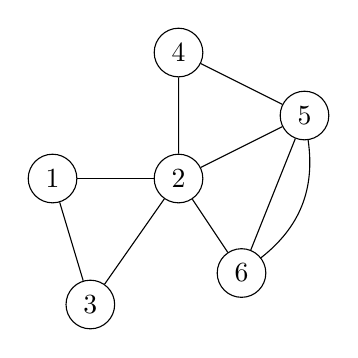
\begin{tikzpicture}[scale=1.6]
            % Nodes
            \node[circle,draw] (A) at (0,0){1};
            \node[circle,draw] (B) at (1,0){2};
            \node[circle,draw] (C) at (0.3,-1){3};
            \node[circle,draw] (D) at (1,1){4};
            \node[circle,draw] (E) at (2,0.5){5};
            \node[circle,draw] (F) at (1.5,-0.75){6};
            % Edges
            \draw (A) -- (B);
            \draw (A) -- (C);
            \draw (C) -- (B);
            \draw (B) -- (D);
            \draw (B) -- (F);
            \draw (B) -- (E);
            \draw (D) -- (E);
            \draw (E) -- (F);
            \path[draw] (E) to[bend right=-30] (F);
        \end{tikzpicture}
        \caption{$G_1 = (N_1,R_1)$.}
        \label{subfig:graph1}
    \end{subfigure}
    \hfill
    \begin{subfigure}[b]{0.3\textwidth}
        \centering
        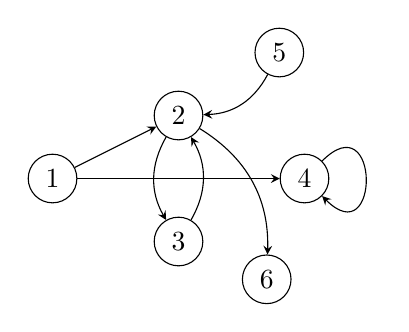
\begin{tikzpicture}[scale=1.6]
            % Nodes
            \node[circle,draw] (A) at (0,0){1};
            \node[circle,draw] (B) at (1, .5){2};
            \node[circle,draw] (C) at (1,-.5){3};
            \node[circle,draw] (D) at (2,0){4};
            \node[circle,draw] (E) at (1.8,1){5};
            \node[circle,draw] (F) at (1.7,-.8){6};
            % Edges
            \path[draw,->,>=stealth] (A) to (D);
            \path[draw,->,>=stealth] (A) to (B);
            \path[draw,->,>=stealth] (E) to[bend left=30] (B);
            \path[draw,->,>=stealth] (B) to[bend right=30] (C);
            \path[draw,->,>=stealth] (B) to[bend left=30] (F);
            \path[draw,->,>=stealth] (C) to[bend right=30] (B);
            \path[draw,->,>=stealth] (D) to[out=45,in=315,looseness=6] (D);
        \end{tikzpicture}
        \caption{$G_2 = (N_2,R_2)$.}
        \label{subfig:graph2}
    \end{subfigure}
    \hfill
    \begin{subfigure}[b]{0.3\textwidth}
        \centering
        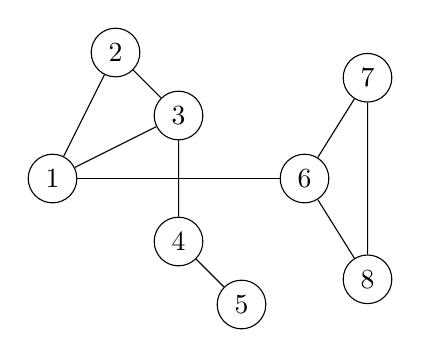
\begin{tikzpicture}[scale=1.6]
            % Nodes
            \node[circle,draw] (A) at (0,0){1};
            \node[circle,draw] (B) at ( .5,1){2};
            \node[circle,draw] (C) at (1, .5){3};
            \node[circle,draw] (D) at (1,-.5){4};
            \node[circle,draw] (E) at (1.5,-1){5};
            \node[circle,draw] (F) at (2,0){6};
            \node[circle,draw] (G) at (2.5,.8){7};
            \node[circle,draw] (H) at (2.5,-.8){8};
            % Edges
            \draw (A) -- (B);
            \draw (A) -- (C);
            \draw (B) -- (C);
            \draw (C) -- (D);
            \draw (D) -- (E);
            \draw (A) -- (F);
            \draw (F) -- (G);
            \draw (F) -- (H);
            \draw (G) -- (H);
        \end{tikzpicture}
        \caption{$G_3 = (N_3,R_3)$.}
        \label{subfig:graph3}
    \end{subfigure}
    \caption{Trois graphes pas trop complexes\dots}
    \label{fig:three-graphs}
 \end{figure}

 \begin{exercise}
     \label{ex:12_exo1}
     Pour chacun de ces graphes $G_i = (V_i, E_i)$, $i=\{1,2,3\}$ de la Figure~\ref{fig:three-graphs}:
     \begin{enumerate}
        \item déterminer les espaces $V_i$ et $E_i$ ;
        %\item déterminer l’ordre de $G_i$ ; 
        \item déterminer les degrés des n\oe uds ;
        %\item déterminer les incidences n\oe uds-arêtes ;
        \item le graphe est-il simple ? Est-il orienté ?
    \end{enumerate}
\end{exercise}

\begin{exercise}
     \label{ex:12_exo5}
     Vérifier si les graphes représentés à la Figure~\ref{fig:12_exo5} possèdent une piste eulérienne. Si oui, possèdent-ils un tour eulérien ?
     \begin{figure}[h!]
         \centering
        \begin{subfigure}[b]{0.3\textwidth}
            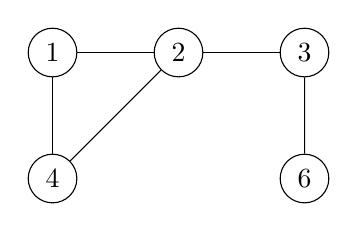
\begin{tikzpicture}[scale=1.6]
                    %NODE
                    \node[circle,draw] (A) at (0,0){1};
                    \node[circle,draw] (B) at (1,0){2};
                    \node[circle,draw] (C) at (2,0){3};
                    \node[circle,draw] (D) at (0,-1){4};
                    \node[circle,draw] (F) at (2,-1){6};
                    
                    %EDGE
                    \draw (A) -- (B);
                    \draw (B) -- (C);
                    \draw (A) -- (D);
                    \draw (D) -- (B);
                    \draw (C) -- (F);
                \end{tikzpicture}
                \caption{$G_1 = (N_1,R_1)$.}
            \label{subfig:graph3}
        \end{subfigure}
        \begin{subfigure}[b]{0.3\textwidth}
            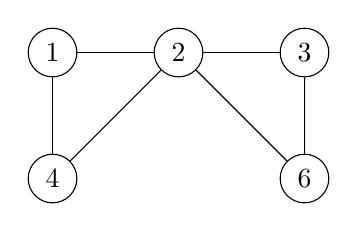
\begin{tikzpicture}[scale=1.6]
                    %NODE
                    \node[circle,draw] (A) at (0,0){1};
                    \node[circle,draw] (B) at (1,0){2};
                    \node[circle,draw] (C) at (2,0){3};
                    \node[circle,draw] (D) at (0,-1){4};
                    \node[circle,draw] (F) at (2,-1){6};
                    
                    %EDGE
                    \draw (A) -- (B);
                    \draw (B) -- (C);
                    \draw (A) -- (D);
                    \draw (B) -- (F);
                    \draw (D) -- (B);
                    \draw (C) -- (F);
                \end{tikzpicture}
                \caption{$G_2 = (N_2,R_2)$.}
            \label{subfig:graph3}
        \end{subfigure}
        \begin{subfigure}[b]{0.3\textwidth}
            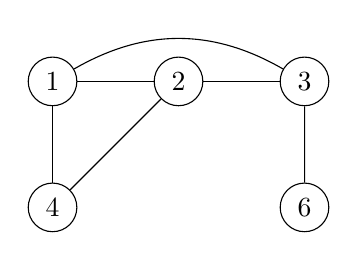
\begin{tikzpicture}[scale=1.6]
                    %NODE
                    \node[circle,draw] (A) at (0,0){1};
                    \node[circle,draw] (B) at (1,0){2};
                    \node[circle,draw] (C) at (2,0){3};
                    \node[circle,draw] (D) at (0,-1){4};
                    \node[circle,draw] (F) at (2,-1){6};
                    
                    %EDGE
                    \draw (A) -- (B);
                    \draw (B) -- (C);
                    \draw (A) -- (D);
                    \draw (D) -- (B);
                    \draw (C) -- (F);
                    \path[draw] (C) to[bend right=30] (A);
                \end{tikzpicture}
                \caption{$G_3 = (N_3,R_3)$.}
            \label{subfig:graph3}
        \end{subfigure}
        \begin{subfigure}[b]{0.3\textwidth}
            \centering
            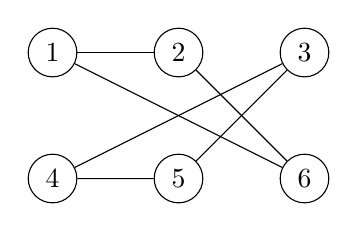
\begin{tikzpicture}[scale=1.6]
                %NODE
                \node[circle,draw] (A) at (0,0){1};
                \node[circle,draw] (B) at (1,0){2};
                \node[circle,draw] (C) at (2,0){3};
                \node[circle,draw] (D) at (0,-1){4};
                \node[circle,draw] (E) at (1,-1){5};
                \node[circle,draw] (F) at (2,-1){6};
                
                %EDGE
                \draw (A) -- (B);
                \draw (A) -- (F);
                \draw (B) -- (F);
                \draw (C) -- (D);
                \draw (C) -- (E);
                \draw (D) -- (E);
            \end{tikzpicture}
            \caption{$G_4 = (N_4,R_4)$.}
            \label{subfig:graph3}
        \end{subfigure}
        \caption{Ces graphes sont ils eulériens ?}
        \label{fig:12_exo5}
     \end{figure}
\end{exercise}

\begin{exercise}
    %TODO : source http://discrete.openmathbooks.org/dmoi2/sec_paths.html
     Vous et vos amis voulez faire le tour du sud-ouest des États-Unis en voiture. Vous visiterez les neuf états représentés à la Figure~\ref{fig:ex6} en suivant une règle pour le moins étrange : vous voulez \emph{absolument} traverser chaque frontière entre états voisins exactement une fois (ainsi, par exemple, vous devez traverser la frontière entre le Colorado et l'Utah exactement une fois). Pouvez-vous le faire ? Si oui, l'endroit où vous commencez votre voyage a-t-il une importance ? Quelle loi mathématique vous permet de conclure ?\footnote{Cet exercice est tiré de : \url{http://discrete.openmathbooks.org/dmoi2/sec_paths.html}}
    \begin{figure}[h!]
        \centering
        \includegraphics[scale=0.5]{content/USA.png}
        \caption{Carte des états sud-ouest des États-Unis d'Amérique (source : \url{http://discrete.openmathbooks.org/dmoi2/sec_paths.html}).}
        \label{fig:ex6}
    \end{figure}
\end{exercise}

\begin{exercise}
    Implémenter le calcul avec l'approche top-down et bottom-up. Laquelle est la plus rapide ? Pourquoi ? \\
    
    On peut aussi utiliser la formule :
    \[
    y_{n, 10} = y_{n - 10, 5} + y_{n - 20, 5} + \dots + y_{n - 5, 2} + y_{n - 10, 2} + \dots
    \]

    Modifier l'implémentation pour utiliser cette formule. Est-ce plus rapide ? Pourquoi ?
\end{exercise}